\section{Methods}
\label{sec:methods}

\subsection{Threat model}
We consider the following adversaries.
\begin{description}
	\item[Network-level adversary] An adversary that monitors at least
		one autonomous system, e.g., ISP, VPS provider, government.
	\item[Relay-level adversary] An adversary that runs at least one Tor relay.
	\item[DNS provider] An adversary that operates the DNS resolver used
		by exit relays, e.g., Google.
	\item[Active] To which extent to we consider active, content-modifying
		adversaries?  Attackers that see DNS can poison response and redirect
		victim to attacker-controlled domain.  That turns problem into trivial,
		classical end-to-end correlation.  Still, probably reason enough to tell
		exit relays that they should use DNSSEC.  Also, we might spot these
		attacks using exitmap.
\end{description}

We do not consider the case where Tor users misconfigure their client and leak
DNS requests unintentionally.

\begin{table}[t]
	\centering
	\begin{tabular}{l r r}
	\toprule
	\textbf{Type} & \textbf{Number of ASs} & \textbf{Percentage} \\
	\midrule
	DNS & 369 & 70.4 \\
	Web & 351 & 67.0 \\
	DNS $\setminus$ Web & 173 & 33.0 \\
	Web $\setminus$ DNS & 155 & 29.6 \\
	DNS $\cap$ Web & 196 & 37.4 \\
	DNS $\cup$ Web & 524 & 100.0 \\
	\bottomrule
	\end{tabular}
	\caption{The set relations between unique traversed ASs for DNS and unique
	traversed ASs for Web.}
	\label{tab:traversed-ass}
\end{table}

\subsection{Exposure at the Exit side}
\begin{itemize}
	\item Rented VPS from OVH, representative for exit relay.
	\item Ran ddptr to Alexa top 1,000 sites.
	\item In total, traversed 30,872 ASs for DNS and 10,707 ASs for web,
		including duplicates.
	\item Eliminating duplicates, we traversed 369 unique DNS ASs and 351 unique
		web ASs.
	\item Among the 369 unique DNS ASes, 173 (46.9\%) were \emph{only} traversed
		for DNS, and not for web.
	\item Among the 351 unique web ASes, 155 (44.2\%) were \emph{only} traversed
		for web, and not for DNS.
	\item 196 ASes were part of both web and DNS ASes.
\end{itemize}

\subsection{Exposure at the Guard side}
\begin{itemize}
	\item Bad guards
	\item recognise dns requests by traffic analysis on the wire.  probably
		difficult because of optimistic data?  can we do more than just timing?
	\item can flow watermarking help?  see houmansadr's
		work~\cite{Houmansadr2011a}
\end{itemize}

\subsection{Mapping DNS resolvers}
Figure~\ref{fig:dnsenum} shows how we can identify an exit relay's DNS resolver.
Over each exit relay, we resolve a unique domain \texttt{PREFIX.tor.nymity.ch}
for which we control the authoritative DNS server.  As a result, we can learn
the IP address of all resolvers that ask for a domain in
\texttt{*.tor.nymity.ch}.

\begin{figure}[t]
	\centering
	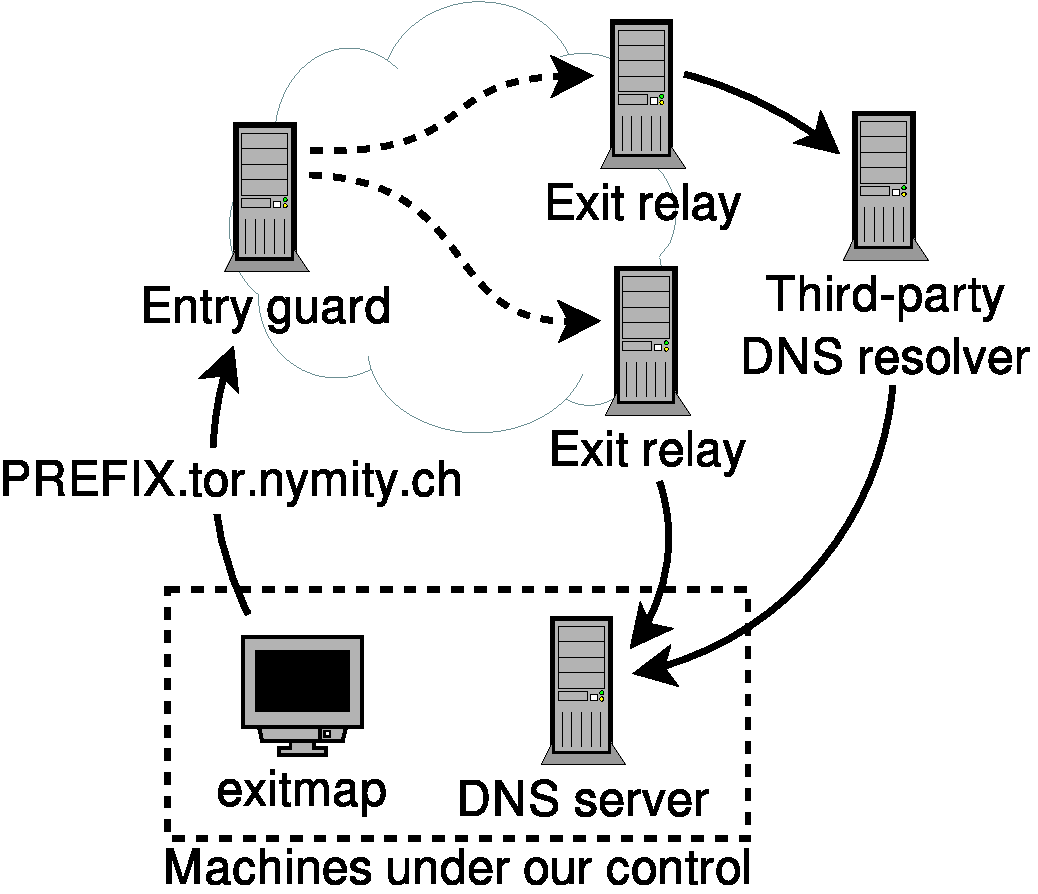
\includegraphics[width=0.8\linewidth]{figures/dns-resolver-enumeration.pdf}
	\caption{Our method to identify the DNS resolver of exit relays.  We resolve
	unique domain names under our control over each exit relay.  We then extract
	the IP address of all resolvers that contacts our DNS server, and map them
	to the respective exit relay.}
	\label{fig:dnsenum}
\end{figure}

An exit relay can either run its own resolver (see the bottom relay in
Fig.~\ref{fig:dnsenum}), or use a third-party resolver such as the one provided
by its ISP (see the top relay in Fig.~\ref{fig:dnsenum}).  If an exit relay runs
its own resolver, we expect to receive a DNS request from the exit relay's IP
address, but if an exit relay uses a third-party resolver, we expect to receive
a request from an unrelated IP address.

We can map DNS requests to exit relays because we encode the relay's 160-bit
unique fingerprint in \texttt{PREFIX}.  We also encode a 40-bit random value in
\texttt{PREFIX} make sure that our requests are not cached anywhere.  As a
result, we send DNS requests of the form
\texttt{FINGERPRINT.RAND.tor.nymity.ch}.

We used the tool exitmap~\cite{Winter2014b} to resolve our domain over all exit
relays.  For performance and reliability, we used only two-hop circuits,
consisting of a static guard relay under our control, and the exit relay.

We ran this experiment from Sep 2015 to Jan 2016, six times a day.

\begin{table}[t]
	\centering
	\begin{tabular}{r l l}
	\toprule
	\textbf{Percentage} & \textbf{Organization} & \textbf{Country} \\
	\midrule
21.6 & Google & US \\ % -> 21.56 bw pct.
13.1 & Local resolver & --- \\ % -> 14.14 bw pct.
6.5 & OpenDNS & US \\ % -> 6.46 bw pct.
6.5 & OVH & FR \\ % -> 6.46 bw pct.
2.7 & S.A.S. & FR \\ % -> 2.65 bw pct.
2.5 & NFOrce Entertainment & NL \\ % -> 2.47 bw pct.
2.1 & UK2 & GB \\ % -> 2.07 bw pct.
2.0 & Iomart & GB \\ %  -> 1.96 bw pct.
1.9 & CYBERDYNE & LR \\ % -> 1.90 bw pct.
1.7 & DFRI & SE \\ % -> 1.74 bw pct.
% 1.7 & Level 3 Communications & US \\ % -> 1.72 bw pct.

% 	306 & 33.4\% & Google & US \\
% 	62 & 6.8\% & OVH SAS & FR \\
% 	26 & 2.8\% & OpenDNS & US \\
% 	23 & 2.5\% & Hetzner Online & DE \\
% 	18 & 2.0\% & S.A.S. & FR \\
% 	17 & 1.9\% & Hurricane Electric & US \\
% 	14 & 1.5\% & LeaseWeb Netherlands & NL \\
% 	12 & 1.3\% & Level 3 Communications & US \\
% 	8 & 0.9\% & Iomart & GB \\
% 	7 & 0.8\% & PlusServer & DE \\
% 	\hline
% 	71 & 7.7\% & Local resolver & \\
	\bottomrule
	\end{tabular}
	\caption{The top ten resolvers used by all exit relays by capacity on Jan 1,
	2016.  More than 20\% of all exit bandwidth at the time used Google's DNS
	server.  13.1\% of exit bandwidth is resolved by local DNS resolvers.}
	\label{tab:dns-resolvers}
\end{table}

\begin{figure}[t]
	\centering
	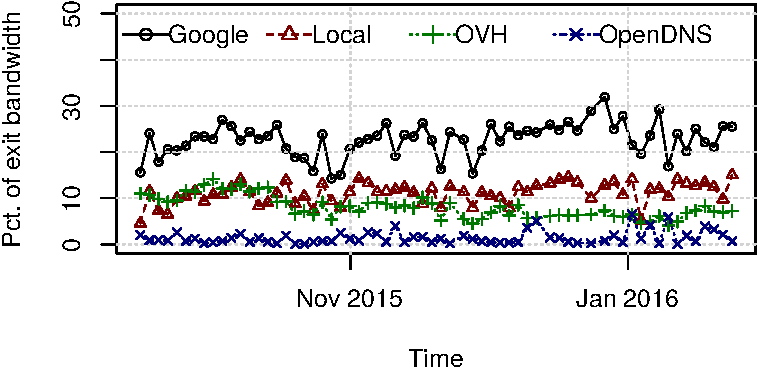
\includegraphics[width=\linewidth]{figures/exit-resolvers.pdf}
	\caption{The amount of the most popular DNS resolvers of exit relays over
	time, weighted by bandwidth.  Google's DNS server is by far the most popular
	resolver of exit relays, followed by a local resolver, OVH, and OpenDNS.}
	\label{fig:exit-resolvers}
\end{figure}

\subsection{Mapping resolver configuration}
In addition to identifying an exit relay's DNS resolver, our technique can
ascertain parts of its configuration.  Resolvers with poor or broken
configuration pose a security risk as attackers could poison or enumerate their
cache.  Therefore, it is important to identify broken resolvers because they
jeopardize the anonymity of Tor users.

\paragraph{Random source ports}
To impede cache poisoning attacks, DNS resolvers should use random source ports
instead of always using UDP port 53.  By inspecting ports, our data allows for
verifying if a given resolver randomizes its source ports.  We classify a
resolver as ``uses randomization'' if the source port does not equal 53.  Note
that this strategy causes a small number of false positives because a
randomizing resolver could use port 53 simply by chance.  However, the
probability of that happening is only $\frac{1}{65535}$.

\paragraph{0x20 encoding}
Resolver can further reduce the chance of cache poisoning by employing 0x20
encoding, i.e., randomizing the capitalization of domain names.  For example,
the domain name foo.com is turned into fOo.CoM, and if the DNS response does not
mirror the randomly chosen capitalization, it is considered unauthentic.  We
classify a resolver as ``uses 0x20'' if it has at least one lowercase and one
uppercase character.  Again, there is a chance of false positives, which depends
on the domain name length.  A 0x20-encoded domain name of $n$ characters
(excluding periods) can be all-uppercase or all-lowercase with probability
$2 \cdot 0.5^n$.

\paragraph{DNSSEC validation}
We can verify if a resolver is validating DNSSEC-signed records by resolving a
domain whose signature is deliberately malformed.  Such a service is provided by
dnssec-failed.org.  A validating resolver would not return an A record while a
non-validating resolver would.  Therefore, we resolve dnssec-failed.org over all
exit relays and check if we get an A record in response.

\subsection{Internet map}
\begin{itemize}
	\item Where do we get our AS and IXP graph from?
	\item Johnson et al.~\cite[\S 5.2]{Johnson2013a} used RouteViews and the CAIDA IPv4
		Routed /24 AS Links Dataset, resulting in 44,605 ASs connected by
		305,381 links.
\end{itemize}

\subsection{Traceroute dataset}
\label{sec:traceroute-dataset}
\begin{itemize}
	\item Find machines that are topologically close to DNS resolvers
		used by exit relays.
	\begin{itemize}
		\item RIPE Atlas probes.
		\item Virtual private systems.
		\item PlanetLab nodes.
		\item Ask exit operators to run traceroutes for us.
	\end{itemize}
	\item Run traceroutes to DNS servers to determine path coverage.
	\item Determine ``AS inflation factor.''
\end{itemize}

\subsection{DNS packet sizes at entry guard}
\begin{itemize}
	\item Send many DNS requests over entry guard.
	\item Capture them on the wire and look at them.
	\item What's the best way to filter out the noise?
\end{itemize}

\subsection{Practical attacks}
We leverage the following building blocks:
\begin{itemize}
	\item Traffic analysis done on an entry guard.  Can DNS requests be isolated
		reliably?
	\item Access to DNS root, .com, and .net.
	\item Ability to use DNS resolver's cache as an oracle.
	\item Ability to enumerate what resolver's an exit relay uses.
	\item Resolvers using EDNS.
	\item Users in country X are likely to resolve domains of country X.
\end{itemize}
